\documentclass{standalone}
\usepackage{tikz}
\usetikzlibrary{patterns, positioning}
\usepackage[sfdefault]{ClearSans} %% option 'sfdefault' activates Clear Sans as the default text font
\usepackage[T1]{fontenc}

\begin{document}
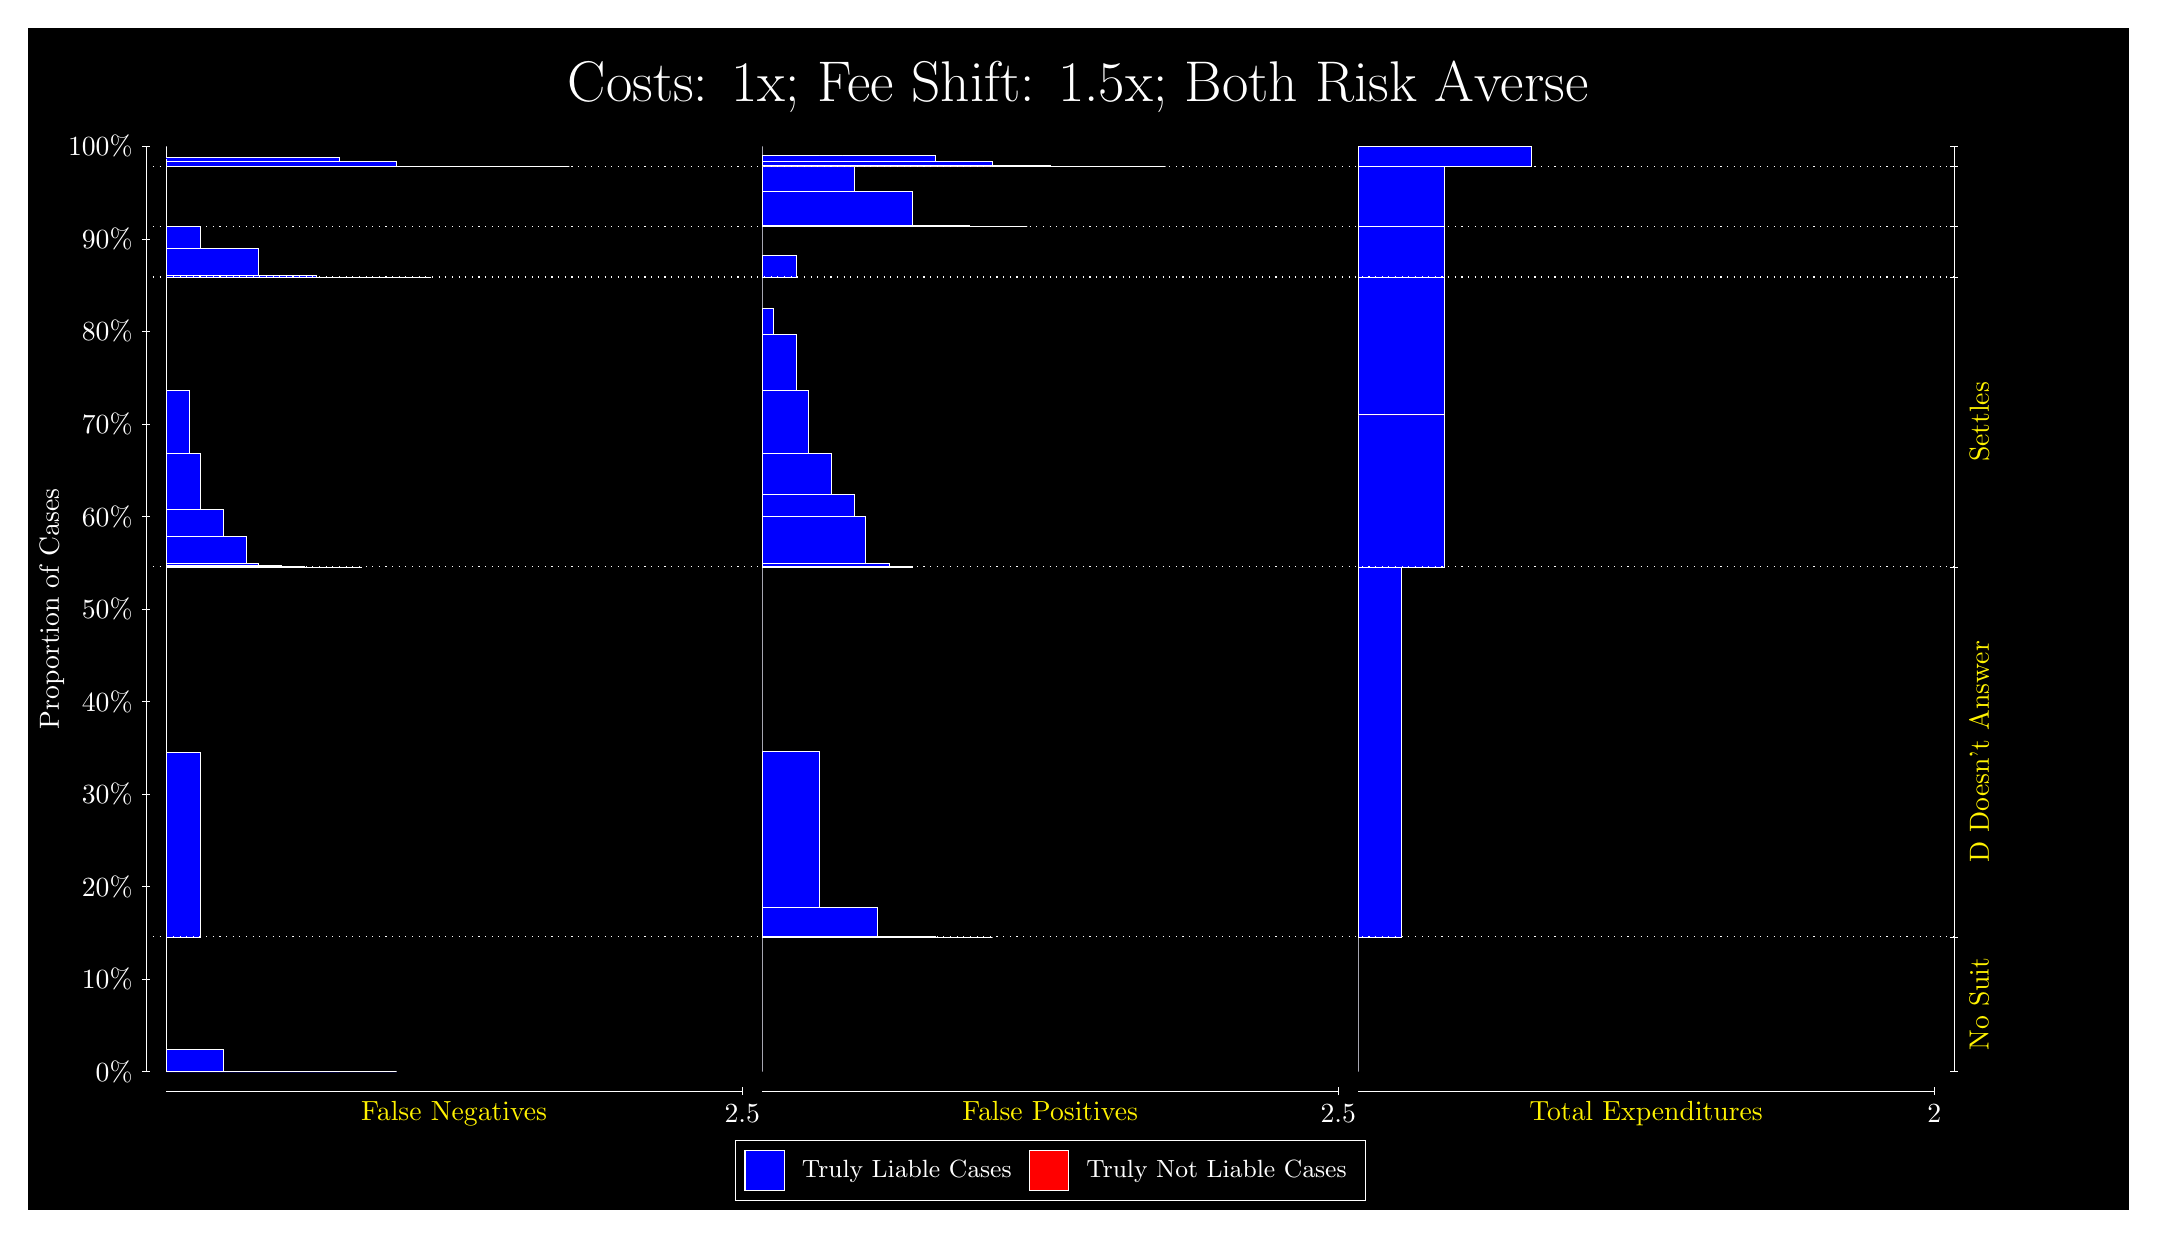
\begin{tikzpicture}
\draw[fill=black] (0,0) rectangle (26.667,15);
\draw[text=white] (0,13.5) rectangle (26.667,15) node[midway] {\huge Costs: 1x; Fee Shift: 1.5x; Both Risk Averse};
\draw[white, very thin] (1.5,1.75) -- (1.5,13.5);
\node[rotate=90, text=white, anchor=center] at (0.3, 7.625) {Proportion of Cases};
\draw[white, very thin] (1.45,1.75) -- (1.55,1.75);
\node[text=white, anchor=east] at (1.45, 1.75) {0\%};
\draw[white, very thin] (1.45,2.925) -- (1.55,2.925);
\node[text=white, anchor=east] at (1.45, 2.925) {10\%};
\draw[white, very thin] (1.45,4.1) -- (1.55,4.1);
\node[text=white, anchor=east] at (1.45, 4.1) {20\%};
\draw[white, very thin] (1.45,5.275) -- (1.55,5.275);
\node[text=white, anchor=east] at (1.45, 5.275) {30\%};
\draw[white, very thin] (1.45,6.45) -- (1.55,6.45);
\node[text=white, anchor=east] at (1.45, 6.45) {40\%};
\draw[white, very thin] (1.45,7.625) -- (1.55,7.625);
\node[text=white, anchor=east] at (1.45, 7.625) {50\%};
\draw[white, very thin] (1.45,8.8) -- (1.55,8.8);
\node[text=white, anchor=east] at (1.45, 8.8) {60\%};
\draw[white, very thin] (1.45,9.975) -- (1.55,9.975);
\node[text=white, anchor=east] at (1.45, 9.975) {70\%};
\draw[white, very thin] (1.45,11.15) -- (1.55,11.15);
\node[text=white, anchor=east] at (1.45, 11.15) {80\%};
\draw[white, very thin] (1.45,12.325) -- (1.55,12.325);
\node[text=white, anchor=east] at (1.45, 12.325) {90\%};
\draw[white, very thin] (1.45,13.5) -- (1.55,13.5);
\node[text=white, anchor=east] at (1.45, 13.5) {100\%};

\draw[white, very thin] (24.457,1.75) -- (24.457,13.5);
\draw[white, very thin] (24.407,1.75) -- (24.507,1.75);
\node[anchor=west] at (24.407, 1.75) {};
\draw[white, very thin] (24.407,3.4602) -- (24.507,3.4602);
\node[anchor=west] at (24.407, 3.4602) {};
\draw[white, very thin] (24.407,8.1583) -- (24.507,8.1583);
\node[anchor=west] at (24.407, 8.1583) {};
\draw[white, very thin] (24.407,11.841) -- (24.507,11.841);
\node[anchor=west] at (24.407, 11.841) {};
\draw[white, very thin] (24.407,12.483) -- (24.507,12.483);
\node[anchor=west] at (24.407, 12.483) {};
\draw[white, very thin] (24.407,13.248) -- (24.507,13.248);
\node[anchor=west] at (24.407, 13.248) {};
\draw[white, very thin] (24.407,13.5) -- (24.507,13.5);
\node[anchor=west] at (24.407, 13.5) {};

\draw[white, very thin, fill=blue] (1.75,1.75) rectangle (4.6775,1.75);
\draw[white, very thin, fill=blue] (1.75,1.75) rectangle (3.9457,1.75);
\draw[white, very thin, fill=blue] (1.75,1.75) rectangle (3.2138,1.7524);
\draw[white, very thin, fill=blue] (1.75,1.7524) rectangle (2.4819,2.03);
\draw[white, very thin, fill=red] (1.75,2.03) rectangle (1.75,2.03);
\draw[white, very thin, fill=blue] (1.75,2.03) rectangle (1.75,3.4602);
\draw[white, very thin, fill=blue] (1.75,3.4602) rectangle (2.1891,5.8063);
\draw[white, very thin, fill=red] (1.75,5.8063) rectangle (1.75,5.8063);
\draw[white, very thin, fill=blue] (1.75,5.8063) rectangle (1.75,8.1583);
\draw[white, very thin, fill=blue] (1.75,8.1583) rectangle (4.2384,8.1583);
\draw[white, very thin, fill=blue] (1.75,8.1583) rectangle (3.9457,8.1583);
\draw[white, very thin, fill=blue] (1.75,8.1583) rectangle (3.6529,8.1583);
\draw[white, very thin, fill=blue] (1.75,8.1583) rectangle (3.5065,8.1683);
\draw[white, very thin, fill=blue] (1.75,8.1683) rectangle (3.2138,8.1774);
\draw[white, very thin, fill=blue] (1.75,8.1774) rectangle (2.921,8.208);
\draw[white, very thin, fill=blue] (1.75,8.208) rectangle (2.7746,8.5521);
\draw[white, very thin, fill=blue] (1.75,8.5521) rectangle (2.4819,8.89);
\draw[white, very thin, fill=blue] (1.75,8.89) rectangle (2.1891,9.597);
\draw[white, very thin, fill=blue] (1.75,9.597) rectangle (2.0428,10.398);
\draw[white, very thin, fill=red] (1.75,10.398) rectangle (1.75,10.398);
\draw[white, very thin, fill=blue] (1.75,10.398) rectangle (1.75,11.841);
\draw[white, very thin, fill=blue] (1.75,11.841) rectangle (5.1167,11.841);
\draw[white, very thin, fill=blue] (1.75,11.841) rectangle (4.3848,11.842);
\draw[white, very thin, fill=blue] (1.75,11.842) rectangle (3.6529,11.863);
\draw[white, very thin, fill=blue] (1.75,11.863) rectangle (2.921,12.206);
\draw[white, very thin, fill=blue] (1.75,12.206) rectangle (2.1891,12.483);
\draw[white, very thin, fill=red] (1.75,12.483) rectangle (1.75,12.483);
\draw[white, very thin, fill=blue] (1.75,12.483) rectangle (2.1891,12.487);
\draw[white, very thin, fill=red] (1.75,12.487) rectangle (1.75,12.487);
\draw[white, very thin, fill=blue] (1.75,12.487) rectangle (1.75,13.248);
\draw[white, very thin, fill=blue] (1.75,13.248) rectangle (6.8732,13.248);
\draw[white, very thin, fill=blue] (1.75,13.248) rectangle (6.1413,13.248);
\draw[white, very thin, fill=blue] (1.75,13.248) rectangle (5.4094,13.251);
\draw[white, very thin, fill=blue] (1.75,13.251) rectangle (4.6775,13.304);
\draw[white, very thin, fill=blue] (1.75,13.304) rectangle (3.9457,13.356);
\draw[white, very thin, fill=blue] (1.75,13.356) rectangle (3.5065,13.356);
\draw[white, very thin, fill=blue] (1.75,13.356) rectangle (3.2138,13.358);
\draw[white, very thin, fill=blue] (1.75,13.358) rectangle (2.7746,13.358);
\draw[white, very thin, fill=blue] (1.75,13.358) rectangle (2.7746,13.358);
\draw[white, very thin, fill=blue] (1.75,13.358) rectangle (2.4819,13.358);
\draw[white, very thin, fill=blue] (1.75,13.358) rectangle (2.0428,13.358);
\draw[white, very thin, fill=blue] (1.75,13.358) rectangle (2.0428,13.363);
\draw[white, very thin, fill=red] (1.75,13.363) rectangle (1.75,13.363);
\draw[white, very thin, fill=blue] (1.75,13.363) rectangle (1.75,13.5);
\draw[white, very thin, fill=red] (9.3189,1.75) rectangle (9.3189,1.75);
\draw[white, very thin, fill=blue] (9.3189,1.75) rectangle (9.3189,3.4602);
\draw[white, very thin, fill=red] (9.3189,3.4602) rectangle (12.246,3.4602);
\draw[white, very thin, fill=blue] (9.3189,3.4602) rectangle (12.246,3.4602);
\draw[white, very thin, fill=blue] (9.3189,3.4602) rectangle (11.515,3.463);
\draw[white, very thin, fill=blue] (9.3189,3.463) rectangle (10.783,3.8354);
\draw[white, very thin, fill=blue] (9.3189,3.8354) rectangle (10.051,5.8121);
\draw[white, very thin, fill=blue] (9.3189,5.8121) rectangle (9.3189,8.1583);
\draw[white, very thin, fill=red] (9.3189,8.1583) rectangle (11.222,8.1583);
\draw[white, very thin, fill=blue] (9.3189,8.1583) rectangle (11.222,8.1681);
\draw[white, very thin, fill=red] (9.3189,8.1681) rectangle (10.929,8.1681);
\draw[white, very thin, fill=blue] (9.3189,8.1681) rectangle (10.929,8.2042);
\draw[white, very thin, fill=red] (9.3189,8.2042) rectangle (10.636,8.2042);
\draw[white, very thin, fill=blue] (9.3189,8.2042) rectangle (10.636,8.7985);
\draw[white, very thin, fill=blue] (9.3189,8.7985) rectangle (10.49,9.0849);
\draw[white, very thin, fill=blue] (9.3189,9.0849) rectangle (10.197,9.6015);
\draw[white, very thin, fill=blue] (9.3189,9.6015) rectangle (9.9044,10.403);
\draw[white, very thin, fill=blue] (9.3189,10.403) rectangle (9.758,11.11);
\draw[white, very thin, fill=blue] (9.3189,11.11) rectangle (9.4652,11.448);
\draw[white, very thin, fill=blue] (9.3189,11.448) rectangle (9.3189,11.841);
\draw[white, very thin, fill=red] (9.3189,11.841) rectangle (9.758,11.841);
\draw[white, very thin, fill=blue] (9.3189,11.841) rectangle (9.758,12.119);
\draw[white, very thin, fill=blue] (9.3189,12.119) rectangle (9.3189,12.483);
\draw[white, very thin, fill=red] (9.3189,12.483) rectangle (12.686,12.483);
\draw[white, very thin, fill=blue] (9.3189,12.483) rectangle (12.686,12.483);
\draw[white, very thin, fill=blue] (9.3189,12.483) rectangle (11.954,12.493);
\draw[white, very thin, fill=blue] (9.3189,12.493) rectangle (11.222,12.924);
\draw[white, very thin, fill=blue] (9.3189,12.924) rectangle (10.49,13.244);
\draw[white, very thin, fill=blue] (9.3189,13.244) rectangle (9.758,13.248);
\draw[white, very thin, fill=red] (9.3189,13.248) rectangle (14.442,13.248);
\draw[white, very thin, fill=blue] (9.3189,13.248) rectangle (14.442,13.248);
\draw[white, very thin, fill=red] (9.3189,13.248) rectangle (13.71,13.248);
\draw[white, very thin, fill=blue] (9.3189,13.248) rectangle (13.71,13.248);
\draw[white, very thin, fill=red] (9.3189,13.248) rectangle (12.978,13.248);
\draw[white, very thin, fill=blue] (9.3189,13.248) rectangle (12.978,13.254);
\draw[white, very thin, fill=red] (9.3189,13.254) rectangle (12.246,13.254);
\draw[white, very thin, fill=blue] (9.3189,13.254) rectangle (12.246,13.311);
\draw[white, very thin, fill=blue] (9.3189,13.311) rectangle (11.515,13.386);
\draw[white, very thin, fill=blue] (9.3189,13.386) rectangle (10.783,13.391);
\draw[white, very thin, fill=red] (9.3189,13.391) rectangle (10.344,13.391);
\draw[white, very thin, fill=blue] (9.3189,13.391) rectangle (10.344,13.391);
\draw[white, very thin, fill=blue] (9.3189,13.391) rectangle (10.051,13.391);
\draw[white, very thin, fill=red] (9.3189,13.391) rectangle (9.6116,13.391);
\draw[white, very thin, fill=blue] (9.3189,13.391) rectangle (9.6116,13.392);
\draw[white, very thin, fill=red] (9.3189,13.392) rectangle (9.3189,13.392);
\draw[white, very thin, fill=blue] (9.3189,13.392) rectangle (9.3189,13.5);
\draw[white, very thin, fill=red] (16.888,1.75) rectangle (16.888,1.75);
\draw[white, very thin, fill=blue] (16.888,1.75) rectangle (16.888,3.4602);
\draw[white, very thin, fill=red] (16.888,3.4602) rectangle (17.437,3.4602);
\draw[white, very thin, fill=blue] (16.888,3.4602) rectangle (17.437,8.1583);
\draw[white, very thin, fill=red] (16.888,8.1583) rectangle (17.986,8.1583);
\draw[white, very thin, fill=blue] (16.888,8.1583) rectangle (17.986,10.092);
\draw[white, very thin, fill=red] (16.888,10.092) rectangle (17.986,10.092);
\draw[white, very thin, fill=blue] (16.888,10.092) rectangle (17.986,11.841);
\draw[white, very thin, fill=red] (16.888,11.841) rectangle (17.986,11.841);
\draw[white, very thin, fill=blue] (16.888,11.841) rectangle (17.986,12.483);
\draw[white, very thin, fill=red] (16.888,12.483) rectangle (17.986,12.483);
\draw[white, very thin, fill=blue] (16.888,12.483) rectangle (17.986,13.248);
\draw[white, very thin, fill=red] (16.888,13.248) rectangle (19.083,13.248);
\draw[white, very thin, fill=blue] (16.888,13.248) rectangle (19.083,13.5);
\draw[white, dotted] (1.5,3.4602) -- (24.457,3.4602);
\draw[white, dotted] (1.5,8.1583) -- (24.457,8.1583);
\draw[white, dotted] (1.5,11.841) -- (24.457,11.841);
\draw[white, dotted] (1.5,12.483) -- (24.457,12.483);
\draw[white, dotted] (1.5,13.248) -- (24.457,13.248);
\draw[white, very thin] (1.75,1.5) -- (9.0689,1.5);
\node[text=yellow, anchor=north] at (5.4094, 1.5) {False Negatives};
\draw[white, very thin] (9.0689,1.45) -- (9.0689,1.55);
\node[text=white, anchor=north] at (9.0689, 1.45) {2.5};

\draw[white, very thin] (9.3189,1.5) -- (16.638,1.5);
\node[text=yellow, anchor=north] at (12.978, 1.5) {False Positives};
\draw[white, very thin] (16.638,1.45) -- (16.638,1.55);
\node[text=white, anchor=north] at (16.638, 1.45) {2.5};

\draw[white, very thin] (16.888,1.5) -- (24.207,1.5);
\node[text=yellow, anchor=north] at (20.547, 1.5) {Total Expenditures};
\draw[white, very thin] (24.207,1.45) -- (24.207,1.55);
\node[text=white, anchor=north] at (24.207, 1.45) {2};

\node[text=yellow, centered, rotate=90] at (24.777, 2.6051) {No Suit};
\node[text=yellow, centered, rotate=90] at (24.777, 5.8092) {D Doesn't Answer};
\node[text=yellow, centered, rotate=90] at (24.777, 9.9999) {Settles};




\draw (12.978300999999998,1.5) node[draw=none] (baseCoordinate) {};
\begin{scope}[align=center]
        \matrix[scale=0.5, draw=white, below=0.5cm of baseCoordinate, nodes={draw}, column sep=0.1cm]{
            \node[rectangle, draw, minimum width=0.5cm, minimum height=0.5cm, fill=blue] {}; &
            \node[draw=none, font=\small, text=white] (B) {Truly Liable Cases}; &
            \node[rectangle, draw, minimum width=0.5cm, minimum height=0.5cm, fill=red] {}; &
            \node[draw=none, font=\small, text=white] (B) {Truly Not Liable Cases}; \\
            };
\end{scope}

\end{tikzpicture}
\end{document}